\documentclass[12pt]{article}
\usepackage{blindtext}
\usepackage[T1]{fontenc}
\usepackage[utf8]{inputenc}
\usepackage{amssymb} % for \smallsetminus
\usepackage{listings}
\usepackage{xcolor}
\usepackage{babel}
\usepackage{caption}
\usepackage{subcaption}
\usepackage{graphicx}
\usepackage{amsmath}
\usepackage{bm}


\title{\Large\vspace{-4cm}Deep Learning for Visual Computing 2020, Assignment 2}

\author{
  Dominik Schörkhuber\\
  \texttt{1027470}
  \and
  Thomas Kaufmann\\
  \texttt{1129115}
}


\date{\today}

\begin{document}
	\maketitle

\section{Part 1 - Optimizers}
In the first part of this assignment we are familiarizing with different optimization algorithms. In Deep Learning we use optimization algorithms, to train the parameters of a neural network. A error (or loss-) function is formulated based on the input and expected output of a network, the optimizer is used to adapt the model parameters such that the loss function is minimized. While Deep Learning problems can typically grow to millions of parameters, we observe in our toy example a 2-dimensional problem space. One can interpret this problem as finding the lowest position on a height map. We visualize the problem space with false color representation, where red areas and blue areas correspond to high values and low values, respectively. 

\subsection{Stochastic Gradient Descent}
We start our investigation with the Stochastic Gradient Descent (SGD) algorithm. Gradient descent refers to stepping along the steepest slope. In the following we describe $L(\theta)$ as the objective function with parameters $\theta$. Gradient descent (like all covered optimization algorithms) works iteratively. In each iteration we compute the velocity $v$ i.e. the change of the parameter vector $\theta$ such that $\theta_{new} = \theta_{old} + v$ whereras $v = \beta v - \alpha \nabla L(\theta)$. For a first analysis we assume $\beta = 0$. As such the speed $v$ is composed of the gradient ($\nabla L(\theta)$) and the learning rate $\alpha$. Higher learning rate means we move further along the gradient in each step, but are therefore less flexible to intermediate changes in the objective function. However, if we set the learning rate too low, the algorithm takes a very long time to converge. Too high learning rate can lead to oscillation as seen in Figure~\ref{fig:sgd_highlr} and Figure~\ref{fig:sgd_lowlr}, respectively.

To increase the speed of convergence we can use the dampening factor $\beta$. Successive movements in the same direction build up higher momentum and allows SGD to take longer steps. The configuration in Figure \ref{fig:sgd_dampening} uses a low dampening factor. Compared to Figure~\ref{fig:sgd_highlr} it converges in 74 steps instead of 216 steps, but slightly overshoots at the left turn due to the built up momentum. The effect of too high momentum is shown in Figure~\ref{fig:sgd_toohighmomentum}. A method to alleviate this is the Nesterov momentum. Instead of computing the gradient at position $\theta$, the gradient is computed at $\theta + v$. This can help because the gradient term always points in the correct direction, while the momentum term may not. This technique severely reduces spiralling around the optimum as shown in Figure~\ref{fig:sgd_nesterov}.

% python optimizer_2d.py fn/camel6.png 500 750 --learning_rate 100000 --beta 0
% python optimizer_2d.py fn/camel6.png 500 750 --learning_rate 1000 --beta 0.9

\begin{figure}
\centering
\begin{subfigure}[b]{.4\linewidth}
% python optimizer_2d.py fn/camel6.png 500 750 --learning_rate 100000 --beta 0 --optimizer SGD
  \centering
  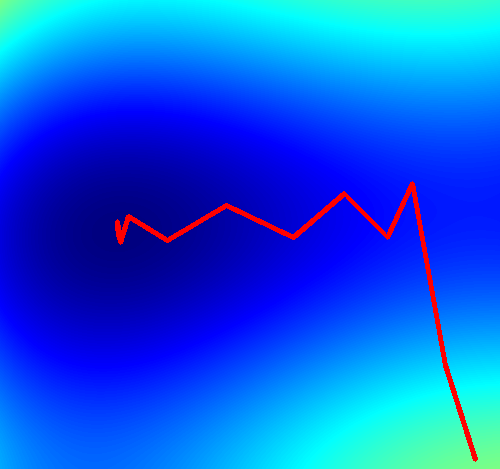
\includegraphics[width=\linewidth]{sgd_nodampening}
  \caption{SGD, $lr=100000$, $\beta=0$}
  \label{fig:sgd_lowlr}
\end{subfigure}
\begin{subfigure}[b]{.4\linewidth}
% python optimizer_2d.py fn/camel6.png 500 750 --learning_rate 10000 --beta 0 --optimizer SGD
% 216 steps
  \centering
  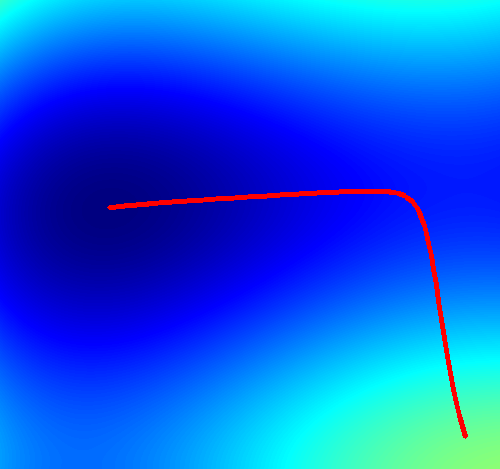
\includegraphics[width=\linewidth]{sgd_nodampening_lowlr}
  \caption{SGD, $lr=10000$, $\beta=0$}
  \label{fig:sgd_highlr}
\end{subfigure}



\begin{subfigure}[b]{.4\linewidth}
% python optimizer_2d.py fn/camel6.png 500 750 --learning_rate 10000 --beta 0.5 --optimizer SGD
% 74 steps
  \centering
  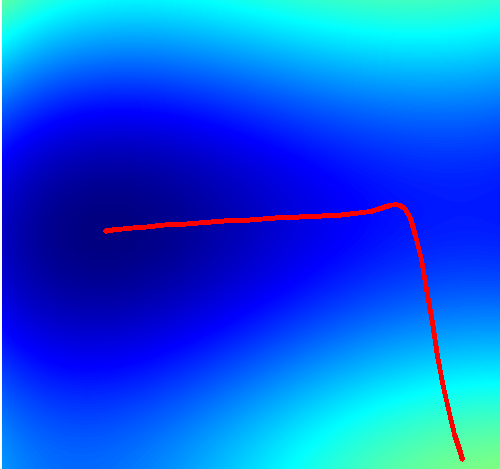
\includegraphics[width=\linewidth]{sgd_moderate_dampening}
  \caption{SGD, $lr=10000$, $\beta=0.5$}
  \label{fig:sgd_dampening}
\end{subfigure}
\begin{subfigure}[b]{.4\linewidth}
% python optimizer_2d.py fn/camel6.png 500 750 --learning_rate 10000 --beta 0.9 --optimizer SGD
  \centering
  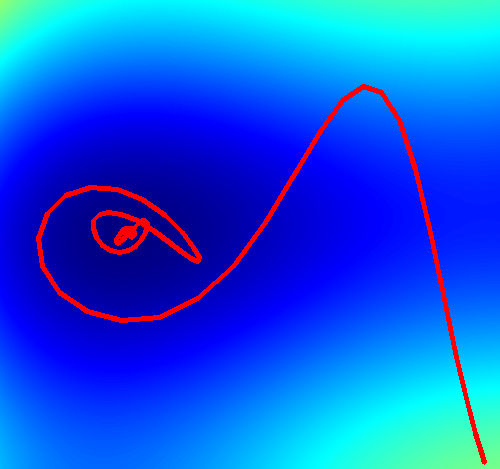
\includegraphics[width=\linewidth]{sgd_highdampening}
  \caption{SGD, $lr=10000$, $\beta=0.9$}
  \label{fig:sgd_toohighmomentum}
\end{subfigure}
\begin{subfigure}[b]{.4\linewidth}
% python optimizer_2d.py fn/camel6.png 500 750 --learning_rate 10000 --beta 0.9 --nesterov --optimizer SGD
  \centering
  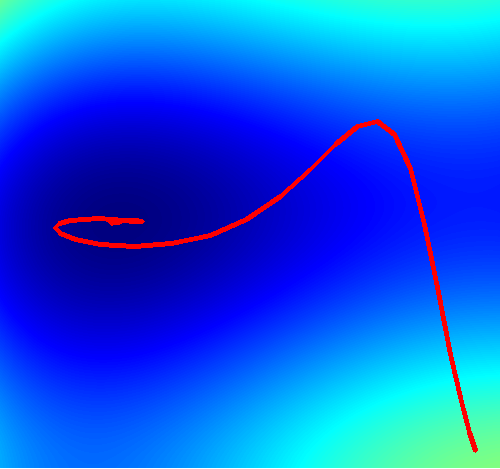
\includegraphics[width=\linewidth]{sgd_nesterov}
  \caption{SGD, $lr=10000$, $\beta=0.9$, with Nesterov momentum}
  \label{fig:sgd_nesterov}
\end{subfigure}

\caption{Shown are different configurations for SGD to emphasize the effect of different parameters.}
\label{fig:sgd_oszillation}
\end{figure}	




\subsection{Adam}
Without going into further detail, Adam maintains not only speed but also velocity with separate dampening factors. Over time dampening increases such 


\subsection{Comparison}



	
\end{document}